\documentclass[
  bibliography=totoc,
  captions=tableheading,
  titlepage=firstiscover,
  twocolumn,
  %10pt,
]{scrartcl}

\setlength{\oddsidemargin}{0.0 cm}
\setlength{\evensidemargin}{0.0 cm}
\setlength{\topmargin}{-1cm}
\setlength{\textheight}{24 cm}
\setlength{\textwidth}{16 cm}

\pagestyle{plain}

\usepackage{fixltx2e}
\usepackage[aux]{rerunfilecheck}
\usepackage{polyglossia}
%\frenchspacing
\setmainlanguage[variant=british]{english}
\usepackage[intlimits]{amsmath}
\usepackage{amssymb}
\usepackage{mathtools}
\usepackage{fontspec}
\setsansfont{Helvetica}
\setmainfont{Charis SIL}
\setmonofont[Scale=0.92]{Source Code Pro}
\defaultfontfeatures{Ligatures=TeX}
\usepackage[
  math-style=ISO,
  bold-style=ISO,
  sans-style=italic,
  nabla=upright,
  partial=upright,
]{unicode-math}
\setmathfont{Tex Gyre Pagella Math}
%\setmathfont{Asana Math}
%\setmathfont{Latin Modern Math}
\setmathfont[range={\mathscr, \mathbfscr}]{XITS Math}
\setmathfont[range=\coloneq]{XITS Math}
\setmathfont[range=\propto]{XITS Math}
\removenolimits{\int}
\let\hbar\relax
\DeclareMathSymbol{\hbar}{\mathord}{AMSb}{"7E}
\DeclareMathSymbol{ℏ}{\mathord}{AMSb}{"7E}
\usepackage[autostyle]{csquotes}
\usepackage[
  locale=US,
  separate-uncertainty=true,
  per-mode=symbol-or-fraction,
]{siunitx}
\usepackage[version=3]{mhchem}
\usepackage{xfrac}
%\usepackage[section, below]{placeins}
\usepackage[
  labelfont=bf,
  font=small,
  width=0.9\textwidth,
]{caption}
\usepackage{subcaption}
\usepackage{graphicx}
\usepackage{grffile}
\usepackage{float}
\usepackage[italic]{hepnicenames}
\floatplacement{figure}{htbp}
\floatplacement{table}{htbp}
\usepackage{booktabs}
\usepackage{pdflscape}
\usepackage[
  sorting=none,
]{biblatex}
\addbibresource{main.bib}
\usepackage{microtype}
\usepackage{blindtext}
\usepackage[
  unicode,
  pdfusetitle,
  pdfcreator={},
  pdfproducer={},
]{hyperref}
\usepackage{bookmark}
\usepackage[shortcuts]{extdash}
\usepackage{tikz}
\captionsetup{width=0.45\textwidth}


\begin{document}

\twocolumn[{%
\begin{center}
  {\LARGE \textbf{\textsf{Top Quark Seminar I}}} \\
  \vspace{1em}
  {\Large \textbf{\textsf{Igor Babuschkin}}} \\
  \vspace{1em}
  {\large \textbf{\textsf{4th January 2015}}}
  \section*{Summary of \enquote{Search for the Top Quark: Results from the DØ Experiment}}
\end{center}
}]

The paper constitutes part of the proceedings of a 1994 high energy physics conference in Glasgow.
It documents the progress that the DØ collaboration had made in the search for the top quark, which at that point had not been discovered, but was strongly suspected to exist.
More precisely, the paper describes an analysis using \SI{13.5}{\per\pico\barn} of integrated luminosity at the Tevatron (a $\Pp\Pap$ collider) which looked for $\Pqt\APqt$ pairs via dilepton plus jets and single leptons plus jets final states.
The preliminary results presented at the conference did not suffice to claim a discovery of the top quark with the necessary statistical significance.

It is interesting to note that, in contrast to the LHC, the dominant \Pqt\!\!\APqt production mechanism at the Tevatron was $q\overline{q}$ annihilation, while gluon fusion had a smaller role.
This was caused by the fact that both protons and antiprotons were collided.

The paper cites \SI{131}{GeV/c^2} as the Standard Model (SM) prediction for the top quark mass $m_{\Pqt}$ at the time.
It also refers to results by the CDF collaboration (TODO: cite) suggesting that the top quark mass would lie in the range \SIrange{160}{190}{GeV/c^2}.

% What characterizes the final states?
% What m_t was expected at the time
% Relation to CDF collaboration

% topological tagging?
% b-quark tagging

\begin{figure}
  \centering
  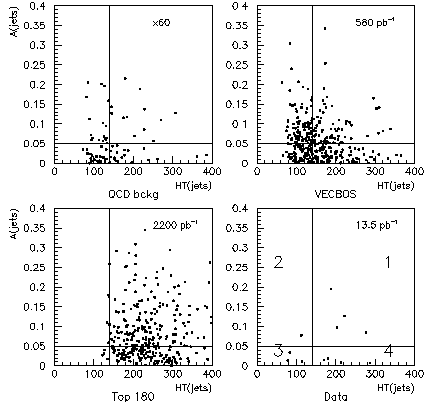
\includegraphics[width=0.5\textwidth]{figures/candidates.pdf}
\end{figure}

\begin{figure}
  \centering
  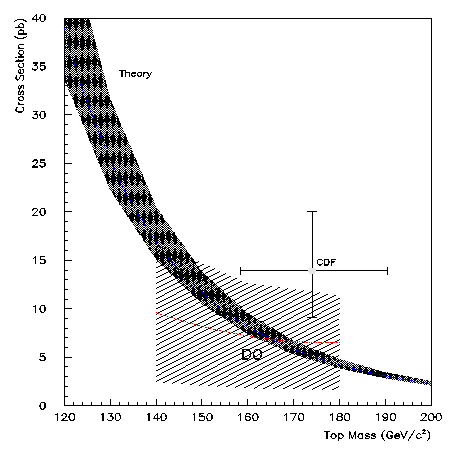
\includegraphics[width=0.5\textwidth]{figures/result.pdf}
\end{figure}

\nocite{*}
\printbibliography

\end{document}
